\section{Energy Storage Sizing Approach} \label{sec:c4_approach}

As mentioned, previous designs of intermittent computing typically adopt a minimised energy storage so as to minimise device dimensions and interruption periods. 
However, such a minimised energy storage leads to frequent save and restore operations, and reduces forward progress.
An appropriate capacitor size instead may balance the three factors. 

We propose a sizing approach which recommends appropriate energy storage capacitance for an ICS, trading off forward progress against capacitor volume and interruption periods. 
We present a system model which accepts real long-term data on environmental energy conditions. 
The three inputs can be swept for design exploration, but we focus on energy storage in this paper. 
The model outputs forward progress, capacitor volume, and interruption periods (defined in Section~\ref{subsec:harvstor}). 
These are subsequently traded off in a cost function to obtain the appropriate energy storage capacitance. 
This process is summarised in \figurename{~\ref{fig:sizingapproach}} with details explained as follows. 

\begin{figure}[!t]
    \centering
    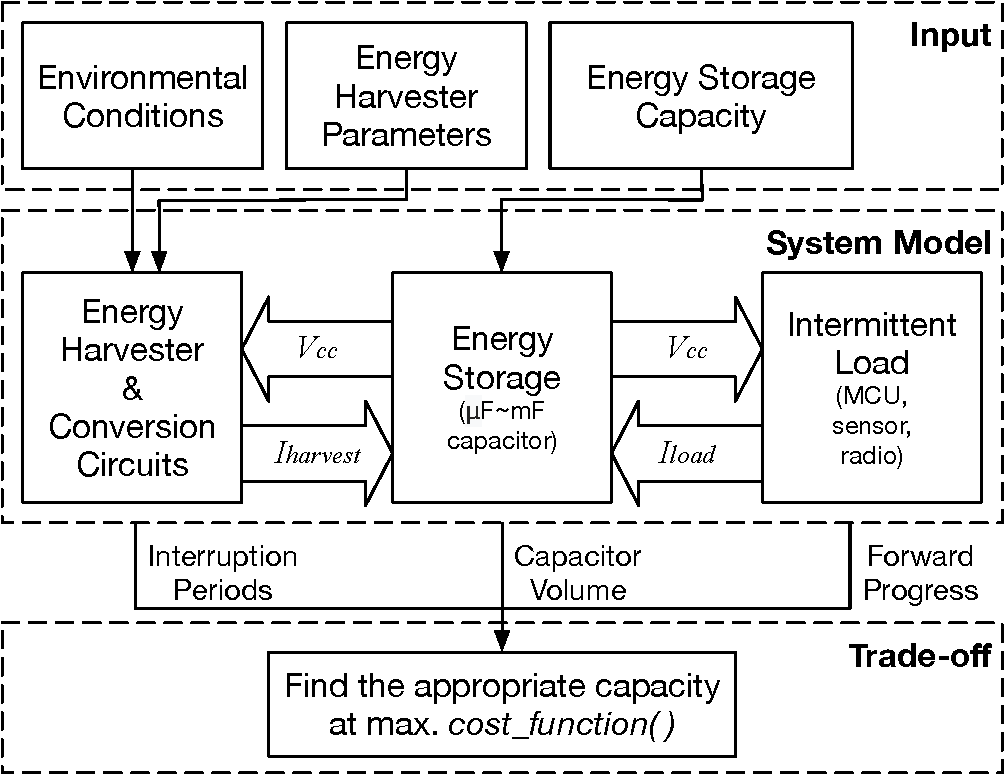
\includegraphics[width=\columnwidth]{ch4_sizingapproach/figures/mdlfrw4}
    \caption{Structure of the proposed system model and sizing approach.}
    \label{fig:sizingapproach}
\end{figure}

    
\subsection{Input}
A time trace of representative environmental energy conditions in the intended deployment location is provided as an input, along with the energy harvester size. 
For design exploration, assuming the energy source is equally distributed in the deployed space, these can optionally be changed to explore variations and scales of harvested power. 
A pre-defined set of energy storage capacitance values are swept through. 

\subsection{System Model}

This contains three modules:
%Design exploration is enabled by changing parameters, for example energy storage and energy harvester sizes.
% As shown in \figurename{~\ref{fig:sizingapproach}}, the system model 
% We provide a system model as further explained in Section~\ref{subsec:systemmodel}. 
%, i.e. \textit{Energy Harvester and Conversion Circuits}, \textit{Energy Storage}, and \textit{Intermittent Load}. The current production $I_{harvest}$ and consumption $I_{load}$ are buffered in the energy storage, which then provides $V_{cc}$ for the load and the harvester output. Due to the variety in each module, they should be individually specified to represent the target platform according to the techniques implemented. 
% The three modules communicate by their voltage and current flows.
\begin{itemize}
    % [topsep=0pt]
    \item \textit{Energy Harvester and Conversion Circuits}: The energy harvester module transduces environmental energy into electricity. 
    % The harvested power is typically conditioned to provide a suitable voltage for charging the energy storage and supplying the load efficiently. 
    In ICSs, conversion circuits may simply be a diode to inhibit backflow of current.
    The energy harvester and conversion circuits can be modelled together as a module because they are usually coupled or integrated. 
    \item \textit{Energy Storage}: Energy storage in ICSs is usually in the form of a \SI{}{\micro\farad}-  to \SI{}{\milli\farad}-scale capacitor. It must be sufficient to complete the most energy-expensive atomic operation, and may be formed only of the decoupling capacitor(s). 
    %provides a minimum energy pulse, which should be set enough
    \item \textit{Intermittent Load}: Includes all the power consumers in an ICS, such as a microcontroller, sensors, and a radio. 
\end{itemize}

The outputs from the system model are the interruption periods, capacitor volume, and forward progress.
% As mentioned, ICS approaches can be classified as static and reactive approaches. These two types of approaches fundamentally differs in how the load consumes power and makes forward progress, and hence require different models for estimating forward progress. Owing to the computing advantage of reactive ICSs as explained in Section~\ref{section:review}, we focus on reactive ICSs for modelling and validation in this paper.
% The unit of energy source conditions should be consistent with the unit of the \textit{Energy Harvester and Conversion Circuits} in the ICS model. 
% Note that the size configuration of energy harvester configures actual dimensions, e.g. PV panel area, while the one of energy storage configures capacitance.
% The size configuration of energy harvester and energy storage can be altered to observe how the design metrics change. 

\subsection{Trade-off}
The appropriate capacitance is then found through a cost function. This may trade off forward progress against capacitor volume and interruption periods.
% The outputs are filtered and any results that fail to meet basic specifications for maximum interruption periods and minimum forward progress are discarded. 


% \begin{itemize}
%     \item [\textbf{S1-}] \textbf{Determine design specifications}: Derive specifications according to a target application, such as minimum forward progress, minimum energy storage capacitance, maximum capacitor dimensions, and maximum interruption periods under certain energy source conditions. 
%     \item [\textbf{S2-}] \textbf{Configure model}: Configure the model as explained in Section~\ref{sec:c2_model} according to the target platform and application, and collect energy source conditions of the environment where the device is deployed. 
%     \item [\textbf{S3-}] \textbf{Size Energy Harvester} With the configured model, run tests with the minimum capacitance, and find the energy harvester size to ensure the minimum forward progress under the given energy source conditions. 
%     \item [\textbf{S4-}] \textbf{Optimise capacitor size}: Generate the relationship between forward progress and capacitance. Evaluate the optimal capacitance by balancing the side effects of capacitor volume and interruption periods with forward progress in a cost function. A cost function is given in Equation~(\ref{eq:tradeoff}):
%     \begin{equation}
%         f = \frac{\alpha_{exe}}{k_1} - (\frac{v_{cap}}{k_2}) ^ {2} - (\frac{T_{recharge}}{k_3}) ^ {2} 
%         \label{eq:tradeoff}
%     \end{equation}
%     where $v_{cap}$ represents capacitor volume and $T_{recharge}$ represents interruption periods. $k_1$, $k_2$, and $k_3$ are linear scalers, which are empirically determined according to design specifications. The negative side effects are calculated in quadratic forms so as to punish high values more heavily. We only consider the above three factors in this paper to size energy storage, but other factors (e.g. dimensions of energy harvesters) can be included.
% \end{itemize}

% \subsection{System Model} \label{subsec:systemmodel}

% As shown in \figurename{~\ref{fig:sizingapproach}}, the system model contains three modules, i.e. \textit{Energy Harvester and Conversion Circuits}, \textit{Energy Storage}, and \textit{Intermittent Load}. The three modules communicate by their voltage and current flows. 
% Due to the variety in each module, the three module should be individually specified to represent the target platform according to the techniques implemented. 

% \subsubsection{Energy Harvester and Conversion Circuits} The energy harvester module transduces environmental energy into electrical power. The harvested power is typically conditioned to provide a suitable voltage for charging the energy storage and supplying the load efficiently. 
% However, in ICSs, such conversion circuits may be omitted, using only a diode to prevent current backflow. The energy harvester and conversion circuits can be modelled together as a module because they are usually coupled and integrated. 

% \subsubsection{Energy Storage} Energy storage in ICSs is usually in the form of a \SI{}{\micro\farad}-  to \SI{}{\milli\farad}-scale capacitor. The energy storage provides the minimum length of an execution period, which should be enough to complete the most energy-expensive atomic operation. 

% \subsubsection{Intermittent Load} The load module includes all the power consumers in an ICS, such as a microcontroller, sensors, and a radio. As mentioned, ICS approaches can be classified as \textit{static} and \textit{reactive}. These two types of approaches fundamentally differs in how the load consumes power and makes forward progress, and hence require different models for estimating forward progress. 

% This framework provides a guide to construct an EHIC system model that estimates forward progress of EHIC devices in real-world deployment. 
% based on an assumption that program progress is linear to effective execution time. 

% The model is driven by energy source conditions as a function of time. 

% This model outputs the time distribution of estimated forward progress over the test period of energy source input. 

% The size of energy harvester dominates the scale of power input. Given a constant source power, the harvested power typically increases with the size of energy harvester. For example, solar panel. 

% \footnote{Here, source power denotes the ambient energy source power exposed to energy harvester in a unit of the energy harvester model input. For example, if the energy harvester model is a photovoltaic (PV) cell model which takes irradiance as input, the source power should be defined in the unit of $W/m^2$. }

% Users should input a source power trace as a representation of the energy source conditions at the deployed site, and then alter the sizes of energy harvester and energy storage to explore the sizing effect on the design specifications. 

% For example, solar power from a solar panel is typically paired with a maximum power point tracking circuit to effectively extract solar power. The model should be configured for the specific energy harvester and the corresponding conversion circuits. 

% Static intermittent computing saves state at pre-installed points, and keeps executing until the supply fails, where the unsaved volatile progress is lost and the device has to re-execute from the last saved point. Reactive intermittent computing only saves state when the supply is about to fail (e.g. when the supply voltage is lower than a threshold), and then enters LPM (stop executing and enter a low-power mode). 
% However, to model intermittent computing is still a challenge due to lack of understanding and abstraction of its behaviours. 
% What is the difference of power consumption between these techniques? Power consumption: computing (CPU), memory R/W, peripherals (radio, ADC, sensor). While peripherals are more application-wise and currently we are not considering this, we focus more on memory R/W and CPU power. Memory R/W is related to both app and int techniques. Computing power, Memory R/W power. 

% \subsubsection{Model Outputs} 
% Define the outputs, e.g. forms, meanings. 
% Outputs come from which model in particular?

% Forward progress: a surface? 
% Dimensions: two (scattered) plots? 
% interruption periods: how do you define interruption periods, charging from where?